\documentclass[a4paper,oneside,12pt]{report}
% Package yang diperlukan
\usepackage{graphicx}      % Untuk memasukkan gambar
\usepackage{geometry}      % Untuk mengatur margin halaman
\usepackage{listings}      % Untuk menampilkan blok kode
\usepackage{xcolor}        % Untuk menggunakan warna
\usepackage{float}         % Untuk kontrol penempatan float (seperti gambar)
\usepackage{hyperref}      % Untuk membuat hyperlink (URL, referensi)
\usepackage{natbib}        % Untuk citation dengan \cite{} yang clickable
\usepackage{indentfirst}   % Untuk memberi indentasi pada paragraf pertama setiap seksi
\usepackage{url}           % Untuk format URL
\usepackage{fancyhdr}      % Untuk kustomisasi header dan footer
\usepackage{tocloft}       % Untuk kustomisasi Daftar Isi
\usepackage{bookmark}      % Untuk manajemen bookmark PDF yang lebih baik

%======================================================================
% PENGATURAN GEOMETRI HALAMAN
%======================================================================
% Margin umum untuk isi laporan
\geometry{left=3cm, right=2.5cm, top=2cm, bottom=2.5cm}
\sloppy

%======================================================================
% PENGATURAN WARNA UNTUK BLOK KODE
%======================================================================
\definecolor{codegreen}{rgb}{0,0.6,0}
\definecolor{codegray}{rgb}{0.5,0.5,0.5}
\definecolor{codepurple}{rgb}{0.58,0,0.82}
\definecolor{backcolour}{rgb}{0.95,0.95,0.92}
\definecolor{darkblue}{rgb}{0,0,0.6}

%======================================================================
% PENGATURAN BLOK KODE (LISTINGS)
%======================================================================
% Gaya umum untuk semua blok kode
\lstdefinestyle{commonstyle}{
    backgroundcolor=\color{backcolour}, 
    breakatwhitespace=false, 
    breaklines=true, 
    captionpos=b, 
    keepspaces=true,
    numbers=left, 
    numbersep=5pt, 
    showspaces=false, 
    showstringspaces=false,
    showtabs=false, 
    tabsize=2, 
    frame=single,
    basicstyle=\ttfamily\footnotesize,
    numberstyle=\tiny\color{codegray},
    columns=flexible,
    postbreak=\mbox{\textcolor{red}{$\hookrightarrow$}\space},
    breakindent=0pt,
    breakautoindent=false
}

% Gaya khusus untuk HTML
\lstdefinestyle{htmlstyle}{
    style=commonstyle,
    language=HTML,
    commentstyle=\color{codegreen},
    keywordstyle=\color{codepurple},
    stringstyle=\color{codegreen},
    basicstyle=\ttfamily\scriptsize
}

% Gaya khusus untuk CSS
\lstdefinestyle{cssstyle}{
    style=commonstyle,
    commentstyle=\color{codegreen},
    keywordstyle=\color{darkblue},
    stringstyle=\color{codepurple},
    emph={color, background, font, margin, padding, border, display, position, width, height},
    emphstyle=\color{darkblue},
    basicstyle=\ttfamily\scriptsize
}

% Gaya khusus untuk Python
\lstdefinestyle{pythonstyle}{
    style=commonstyle,
    language=Python,
    commentstyle=\color{codegreen},
    keywordstyle=\color{darkblue},
    stringstyle=\color{codepurple},
    emph={import,from,class,def,for,while,if,else,elif,try,except,finally},
    emphstyle=\color{darkblue}
}

% Gaya khusus untuk SQL
\lstdefinestyle{sqlstyle}{
    style=commonstyle,
    language=SQL,
    commentstyle=\color{codegreen},
    keywordstyle=\color{darkblue},
    stringstyle=\color{codepurple},
    emph={SELECT,FROM,WHERE,INSERT,UPDATE,DELETE,CREATE,DROP},
    emphstyle=\color{darkblue}
}

% Gaya khusus untuk JavaScript
\lstdefinestyle{javascriptstyle}{
    style=commonstyle,
    language=JavaScript,
    commentstyle=\color{codegreen},
    keywordstyle=\color{darkblue},
    stringstyle=\color{codepurple},
    emph={function,var,let,const,return,if,for,while,do,else,switch,case},
    emphstyle=\color{darkblue}
}

% Gaya khusus untuk Java
\lstdefinestyle{javastyle}{
    style=commonstyle,
    language=Java,
    commentstyle=\color{codegreen},
    keywordstyle=\color{darkblue}\bfseries,
    stringstyle=\color{codepurple},
    emph={@Test,@Mock,@InjectMocks,@ExtendWith},
    emphstyle=\color{codepurple}
}

%======================================================================
% PENGATURAN LAIN-LAIN
%======================================================================

% Mengganti nama default "Figure" menjadi "Gambar"
\renewcommand{\figurename}{Gambar}
\renewcommand{\thefigure}{\arabic{figure}}

% Pengaturan Hyperlink
\hypersetup{
    colorlinks=true, 
    linkcolor=black, 
    filecolor=black, 
    urlcolor=black,
    citecolor=blue,
    pdftitle={Laporan Praktikum}, 
    pdfpagemode=FullScreen, 
    breaklinks=true
}

% Pengaturan citation style
\bibliographystyle{plain}

% Pengaturan Header & Footer (nomor halaman di tengah bawah)
\pagestyle{fancy}
\fancyhf{}
\fancyfoot[C]{\thepage}
\renewcommand{\headrulewidth}{0pt}

\fancypagestyle{plain}{
    \fancyhf{}
    \fancyfoot[C]{\thepage}
    \renewcommand{\headrulewidth}{0pt}
}

%======================================================================
% PENGATURAN STRUKTUR BAB DAN DAFTAR ISI
%======================================================================
\renewcommand{\contentsname}{Daftar Isi}
\renewcommand{\bibname}{Daftar Pustaka}

% Menghilangkan nomor bab tetapi mempertahankan penomoran seksi
\renewcommand{\thechapter}{}
\renewcommand{\chaptername}{}

% Format penomoran seksi menjadi [nomor bab].[nomor seksi]
\renewcommand{\thesection}{\arabic{chapter}.\arabic{section}}
\renewcommand{\thesubsection}{\thesection.\arabic{subsection}}

\setcounter{secnumdepth}{3}
\setcounter{tocdepth}{2}

% Format Daftar Isi (TOC)
\renewcommand{\cftchapdotsep}{\cftdotsep}
\renewcommand{\cftchapleader}{\cftdotfill{\cftchapdotsep}}
\setlength{\cftchapindent}{0em}
\setlength{\cftsecindent}{2em}
\setlength{\cftsubsecindent}{4em}
\setlength{\cftchapnumwidth}{0em}
\setlength{\cftsecnumwidth}{2.5em}
\setlength{\cftsubsecnumwidth}{3.2em}
\renewcommand{\cftchappresnum}{}
\renewcommand{\cftchapaftersnum}{}

% Perintah kustom untuk membuat judul bab di TOC menjadi tebal
\newcommand{\tocboldsection}[1]{%
  \protect\renewcommand{\protect\cftchapfont}{\protect\bfseries}%
  #1%
  \protect\renewcommand{\protect\cftchapfont}{}%
}

%======================================================================
% AWAL DOKUMEN
%======================================================================
\begin{document}

% Halaman Judul
\newgeometry{left=3cm, right=2.5cm, top=2.5cm, bottom=3cm}
\begin{titlepage}
\begin{center}
\vspace*{0.5cm}
{\large \textbf{\MakeUppercase{Laporan Praktikum}}} \\[0.4cm]
{\large \textbf{\MakeUppercase{PRAKTIKUM PENGUJIAN PERANGKAT LUNAK}}} \\[0.4cm]
{\large \textbf{\MakeUppercase{Pertemuan 8}}} \\[0.4cm]
{\large \textbf{\MakeUppercase{AUTOMATION TESTING: WEB ELEMENT LOCATORS}}} \\[1.5cm]


\includegraphics[height=7cm]{lambang ugm.png} \\[1cm]

{\normalsize \textbf{Disusun oleh:}} \\[0.4cm]
\begin{tabular}{@{}l l @{}}
  \textbf{Nama}           & : Januarsyah Akbar \\
  \textbf{NIM}            & : 24/535846/SV/24314 \\
  \textbf{Kelas}          & : PL4B2 \\
    \textbf{Dosen Pengampu} & : Divi Galih Prasetyo Putri, S.Kom., M.Kom., Ph.D.
\end{tabular} \\[1.2cm]

{\normalsize \textbf{PROGRAM STUDI D-IV}} \\[0.2cm]
{\normalsize \textbf{TEKNOLOGI REKAYASA PERANGKAT LUNAK}} \\[0.2cm]
{\normalsize \textbf{DEPARTEMEN TEKNIK ELEKTRO DAN INFORMATIKA}} \\[0.2cm]
{\normalsize \textbf{SEKOLAH VOKASI}} \\[0.2cm]
{\normalsize \textbf{UNIVERSITAS GADJAH MADA}} \\[0.2cm]
{\normalsize \textbf{YOGYAKARTA}} \\[0.2cm]
{\normalsize \textbf{\today}} \\[1.2cm]
\end{center}
\end{titlepage}
\restoregeometry

\thispagestyle{empty}
\clearpage
\stepcounter{page}
\thispagestyle{empty}

% --- Daftar Isi ---
\addcontentsline{toc}{chapter}{Daftar Isi}
\tableofcontents
\clearpage

% Mengatur penomoran halaman menjadi arab dan mulai dari 3
\pagenumbering{arabic}
\setcounter{page}{3}

%======================================================================
\chapter[Tujuan Praktikum]{Tujuan Praktikum}
%======================================================================
\begin{enumerate}
    \item Mahasiswa mampu memahami berbagai teknik lokator elemen web.
    \item Mahasiswa mampu mengimplementasikan pencarian elemen menggunakan berbagai tipe locators seperti Name, XPath, dan Tag Name pada pengujian antarmuka dengan Selenium WebDriver.
\end{enumerate}
\clearpage

%======================================================================
\chapter[\texorpdfstring{\tocboldsection{Hasil dan Pembahasan}}{Hasil dan Pembahasan}]{Hasil dan Pembahasan}
%======================================================================

%----------------------------------------------------------------------
\section{Tugas}
%----------------------------------------------------------------------

Berikut adalah penjelasan dan tahap praktikum untuk pembuatan dan eksekusi \textit{Automated Testing} terhadap interaksi aplikasi spesifik, yakni portal SauceDemo menggunakan berbagai tipe \textit{Web Element Locators}. Pengujian dilakukan berdasarkan skenario \textit{test case login} dengan langkah-langkah sebagai berikut:

\begin{enumerate}
    \item Mengecek keberadaan teks ``Swag Labs''.
    \item Mengecek keberadaan \textit{field} \texttt{username}.
    \item Membersihkan (\textit{clear}) \textit{field} \texttt{username}.
    \item Mengisi \textit{field} \texttt{username}.
    \item Mengecek keberadaan \textit{field} \texttt{password}.
    \item Membersihkan (\textit{clear}) \textit{field} \texttt{password}.
    \item Mengisi \textit{field} \texttt{password}.
    \item Mengecek keberadaan tombol \textit{login}.
    \item Melakukan klik pada tombol \textit{login}.
\end{enumerate}

\subsection{Pengujian Login SauceDemo Sederhana (\texttt{SauceDemoLoginTest.java})}
Pada bagian ini, kita akan membuat kelas \texttt{SauceDemoLoginTest} untuk memverifikasi proses \textit{login} dengan mencari elemen-elemennya menggunakan locators spesifik seperti Name, XPath, dan Tag Name.

\subsubsection*{1. Mendefinisikan Package dan Import}
Langkah pertama adalah melakukan \textit{import library} yang dibutuhkan dari Selenium WebDriver dan JUnit 5:

\begin{lstlisting}[style=javastyle, caption=Import Dependencies]
import org.junit.jupiter.api.AfterEach;
import org.junit.jupiter.api.BeforeEach;
import org.junit.jupiter.api.Test;
import org.openqa.selenium.By;
import org.openqa.selenium.WebDriver;
import org.openqa.selenium.WebElement;
import org.openqa.selenium.safari.SafariDriver;

import static org.junit.jupiter.api.Assertions.*;
\end{lstlisting}

\subsubsection*{2. Persiapan WebDriver (Setup)}
Selanjutnya, kita mendefinisikan kelas pengujian dan melakukan persiapan awal menggunakan anotasi \texttt{@BeforeEach}. Inisialisasi \textit{browser} menggunakan \texttt{SafariDriver}.

\begin{lstlisting}[style=javastyle, caption=Inisialisasi Kelas dan Setup WebDriver]
public class SauceDemoLoginTest {

    private WebDriver driver;

    @BeforeEach
    public void setUp() {
        driver = new SafariDriver();
    }
\end{lstlisting}

\subsubsection*{3. Helper Methods untuk Pencarian Elemen}
Untuk menghindari repetisi serta \textit{error} yang tak tertangani, dibuat helper method \texttt{find} untuk menyederhanakan pencarian elemen dan \texttt{isPresent} untuk mengecek apakah elemen muncul.

\begin{lstlisting}[style=javastyle, caption=Helper Method]
    private WebElement find(By locator) {
        return driver.findElement(locator);
    }

    private boolean isPresent(By locator) {
        try {
            return !driver.findElements(locator).isEmpty();
        } catch (Exception e) {
            return false;
        }
    }
\end{lstlisting}

\subsubsection*{4. Skenario Pengujian Login dengan Beragam Locator}
Skenario utama mengarahkan web driver ke laman SauceDemo dan menggunakan locators untuk melakukan interaksi. \texttt{By.xpath} digunakan untuk validasi teks header. \texttt{By.name} dipakai untuk input username. Sedangkan password ditemukan menggunakan \textit{XPath axes} (\texttt{following}). Terakhir, \texttt{By.tagName} diiterasikan untuk mencari tombol berjenis \texttt{submit}.

\begin{lstlisting}[style=javastyle, caption=Test Method Login Locator]
    @Test
    public void testLogin() {
        driver.get("https://www.saucedemo.com/");
        
        // 1) cek text "Swag Labs" ada menggunakan XPath (text node)
        By swagText = By.xpath("//*[text()='Swag Labs']");
        assertTrue(isPresent(swagText), "Swag Labs text should be present");

        // 2) cek field username ada (gunakan locator by NAME)
        By usernameBy = By.name("user-name");
        assertTrue(isPresent(usernameBy), "Username field should be present");
        
        WebElement usernameInput = find(usernameBy);
        usernameInput.clear();
        usernameInput.sendKeys("standard_user");

        // 3) cek field password menggunakan XPath dengan axes
        By passwordBy = By.xpath("//input[@name='user-name']/following::input[@type='password'][1]");
        assertTrue(isPresent(passwordBy), "Password field should be present");
        
        WebElement passwordInput = find(passwordBy);
        passwordInput.clear();
        passwordInput.sendKeys("secret_sauce");

        // 4) cek tombol login menggunakan TAG / collection approach
        java.util.List<WebElement> inputs = driver.findElements(By.tagName("input"));
        WebElement loginButton = null;
        for (WebElement el : inputs) {
            String type = el.getAttribute("type");
            if (type != null && (type.equalsIgnoreCase("submit") || type.equalsIgnoreCase("button"))) {
                loginButton = el;
                break;
            }
        }
        assertNotNull(loginButton, "Login button should be present");
        
        loginButton.click();

        String currentUrl = driver.getCurrentUrl();
        assertEquals("https://www.saucedemo.com/inventory.html", currentUrl);
    }
\end{lstlisting}

\begin{figure}[H]
    \centering
    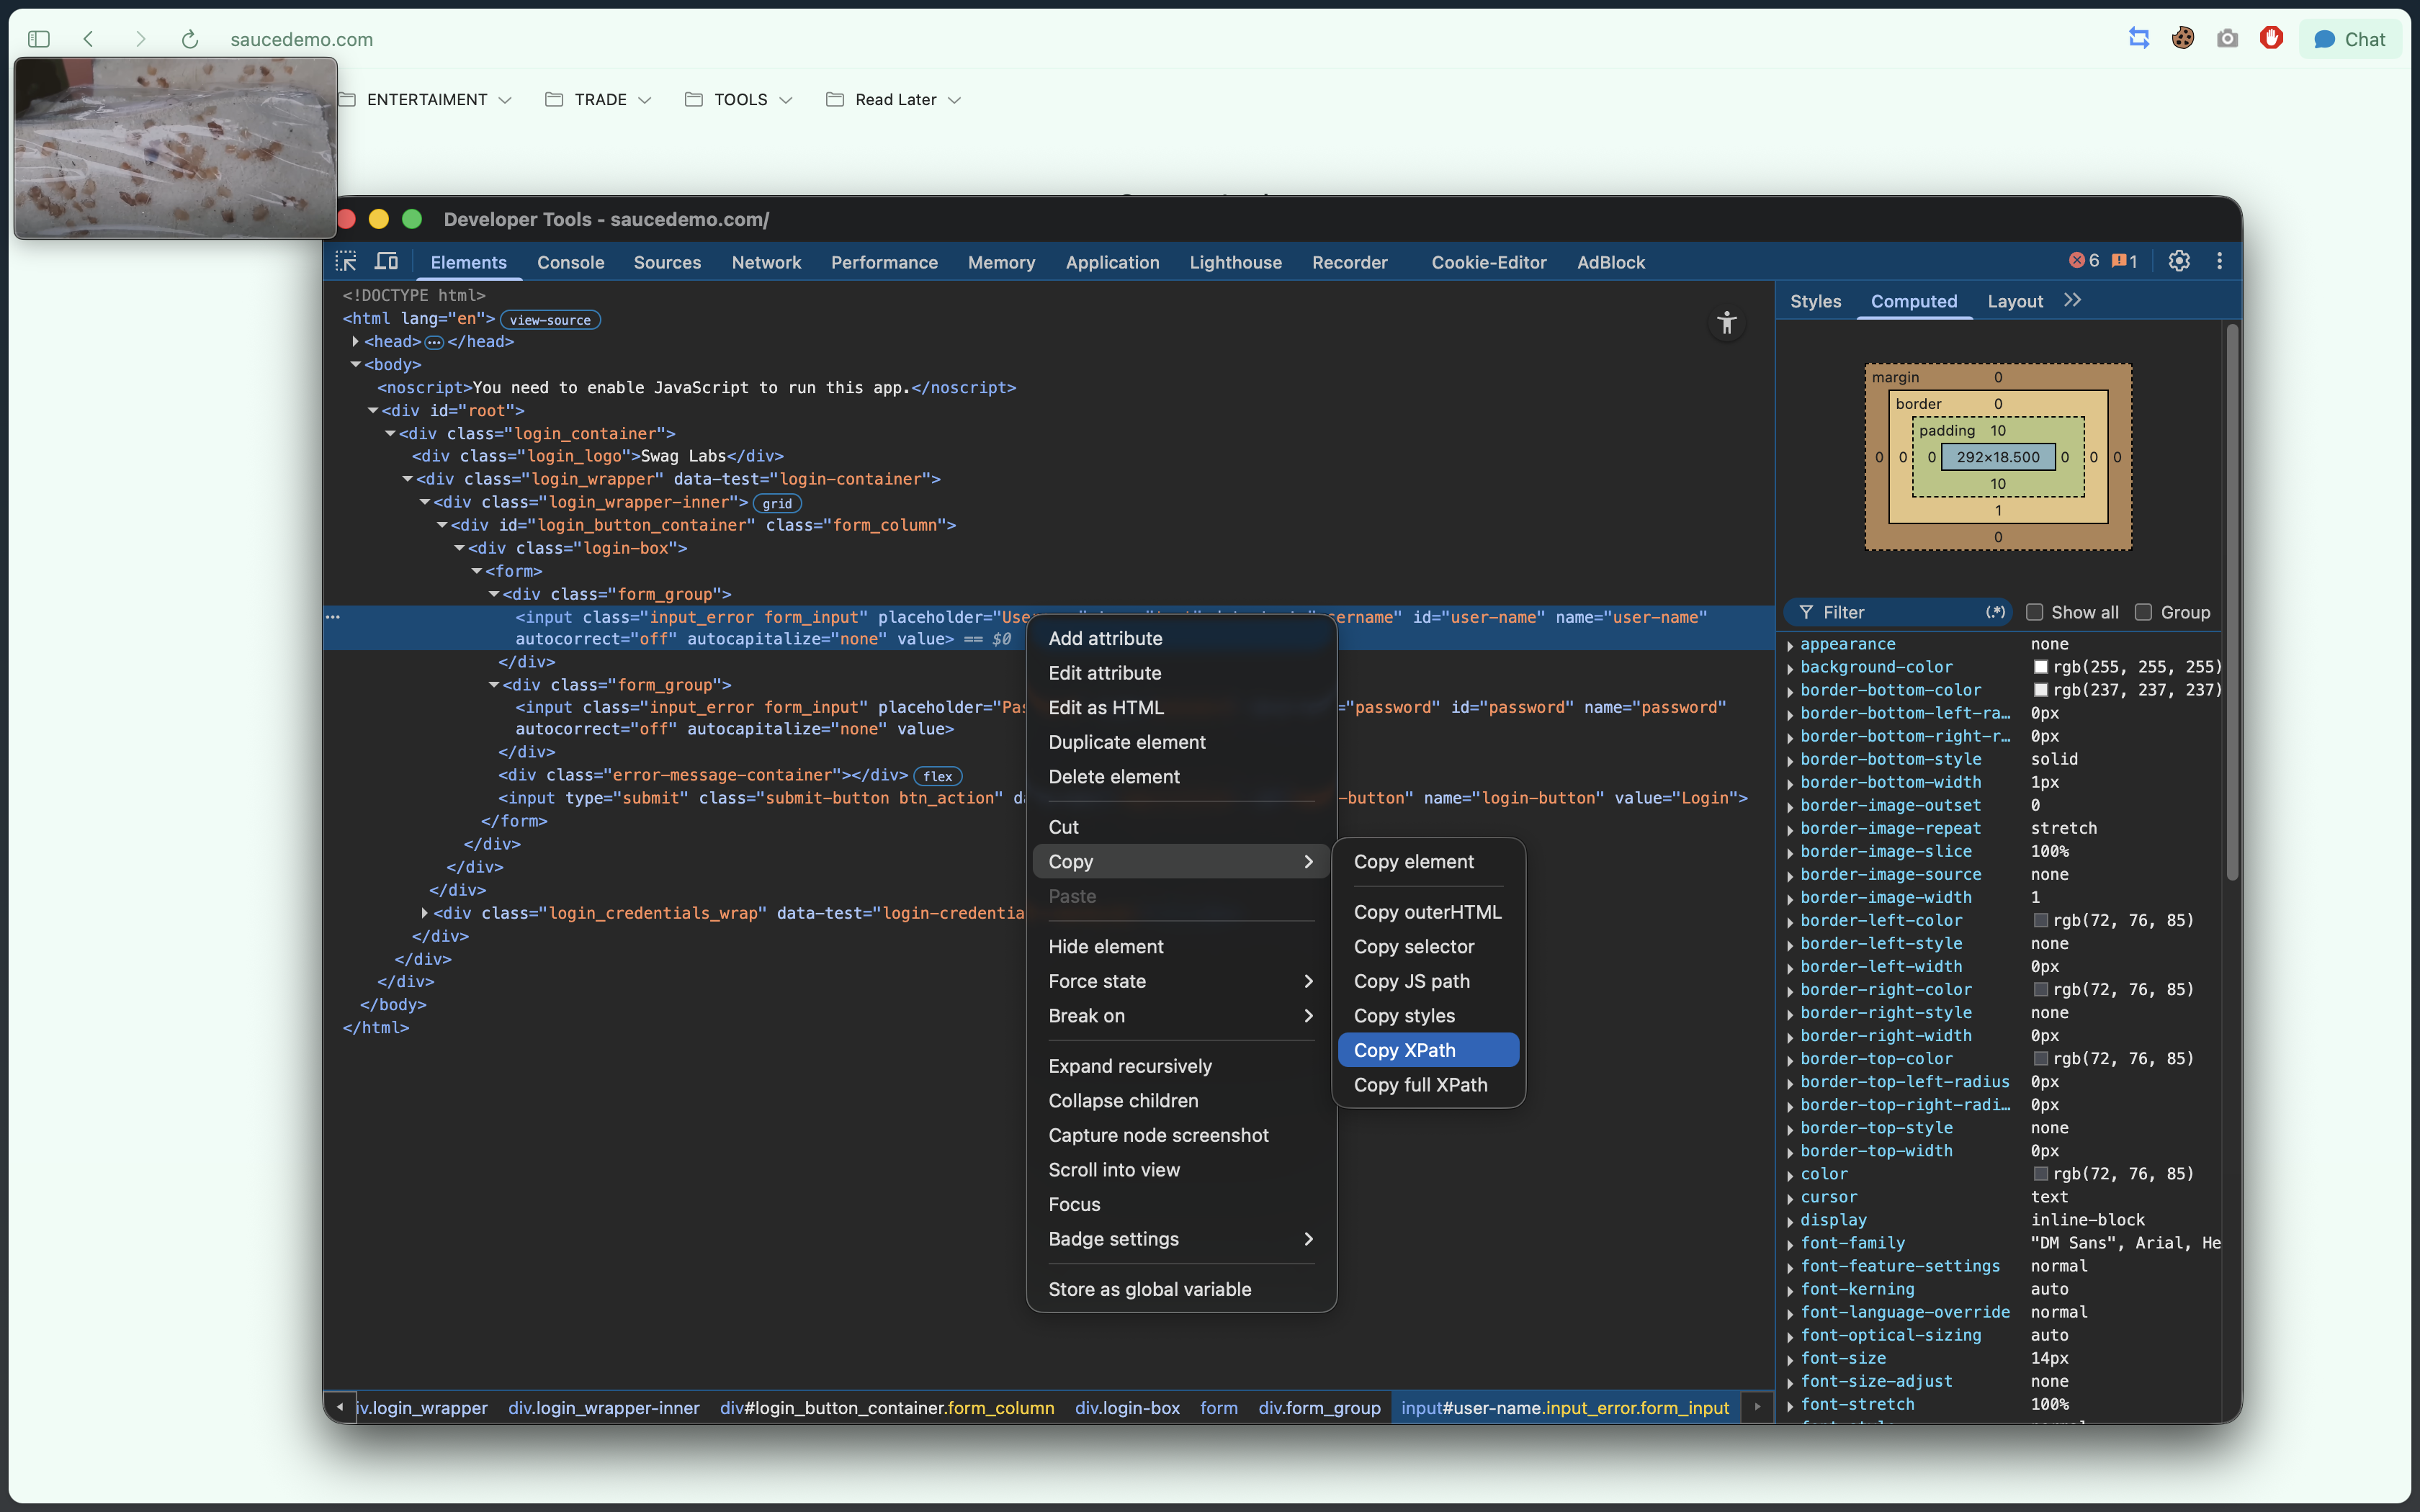
\includegraphics[width=0.9\textwidth]{screenshot step/xpath.png}
    \caption{Penerapan Locators Menggunakan XPath, Name, dan TagName}
\end{figure}

\subsubsection*{5. Membersihkan WebDriver (Teardown)}
Bagian terakhir menggunakan anotasi \texttt{@AfterEach} ditujukan untuk mengakhiri sesi \textit{browser} secara aman:

\begin{lstlisting}[style=javastyle, caption=Penutupan Sesi Browser]
    @AfterEach
    public void tearDown() {
        if (driver != null) {
            driver.quit();
        }
    }
}
\end{lstlisting}

\subsubsection*{Hasil Test}
Berikut adalah tampilan interaksi sukses yang mengkonfirmasi \textit{locators} berhasil menjangkau komponen front-end aplikasi web tersebut.

\begin{figure}[H]
    \centering
    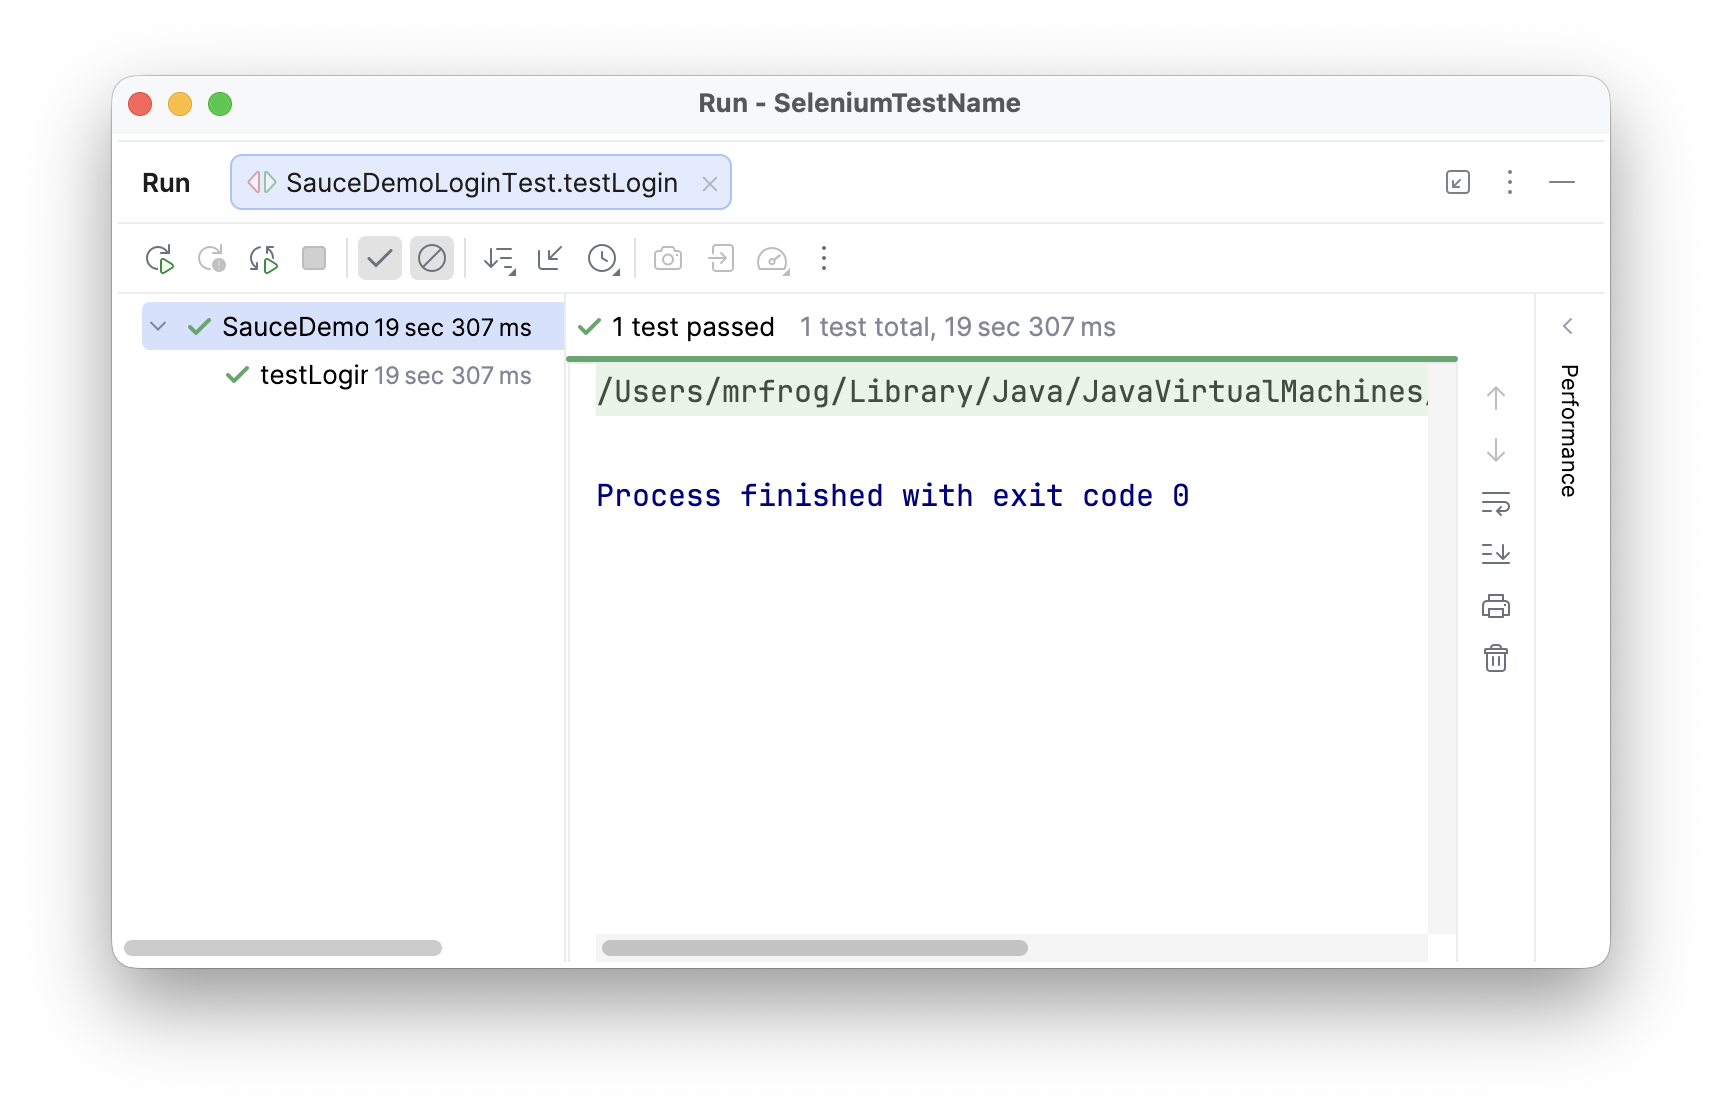
\includegraphics[width=0.9\textwidth]{screenshot step/logintest.png} \\[0.5cm]
    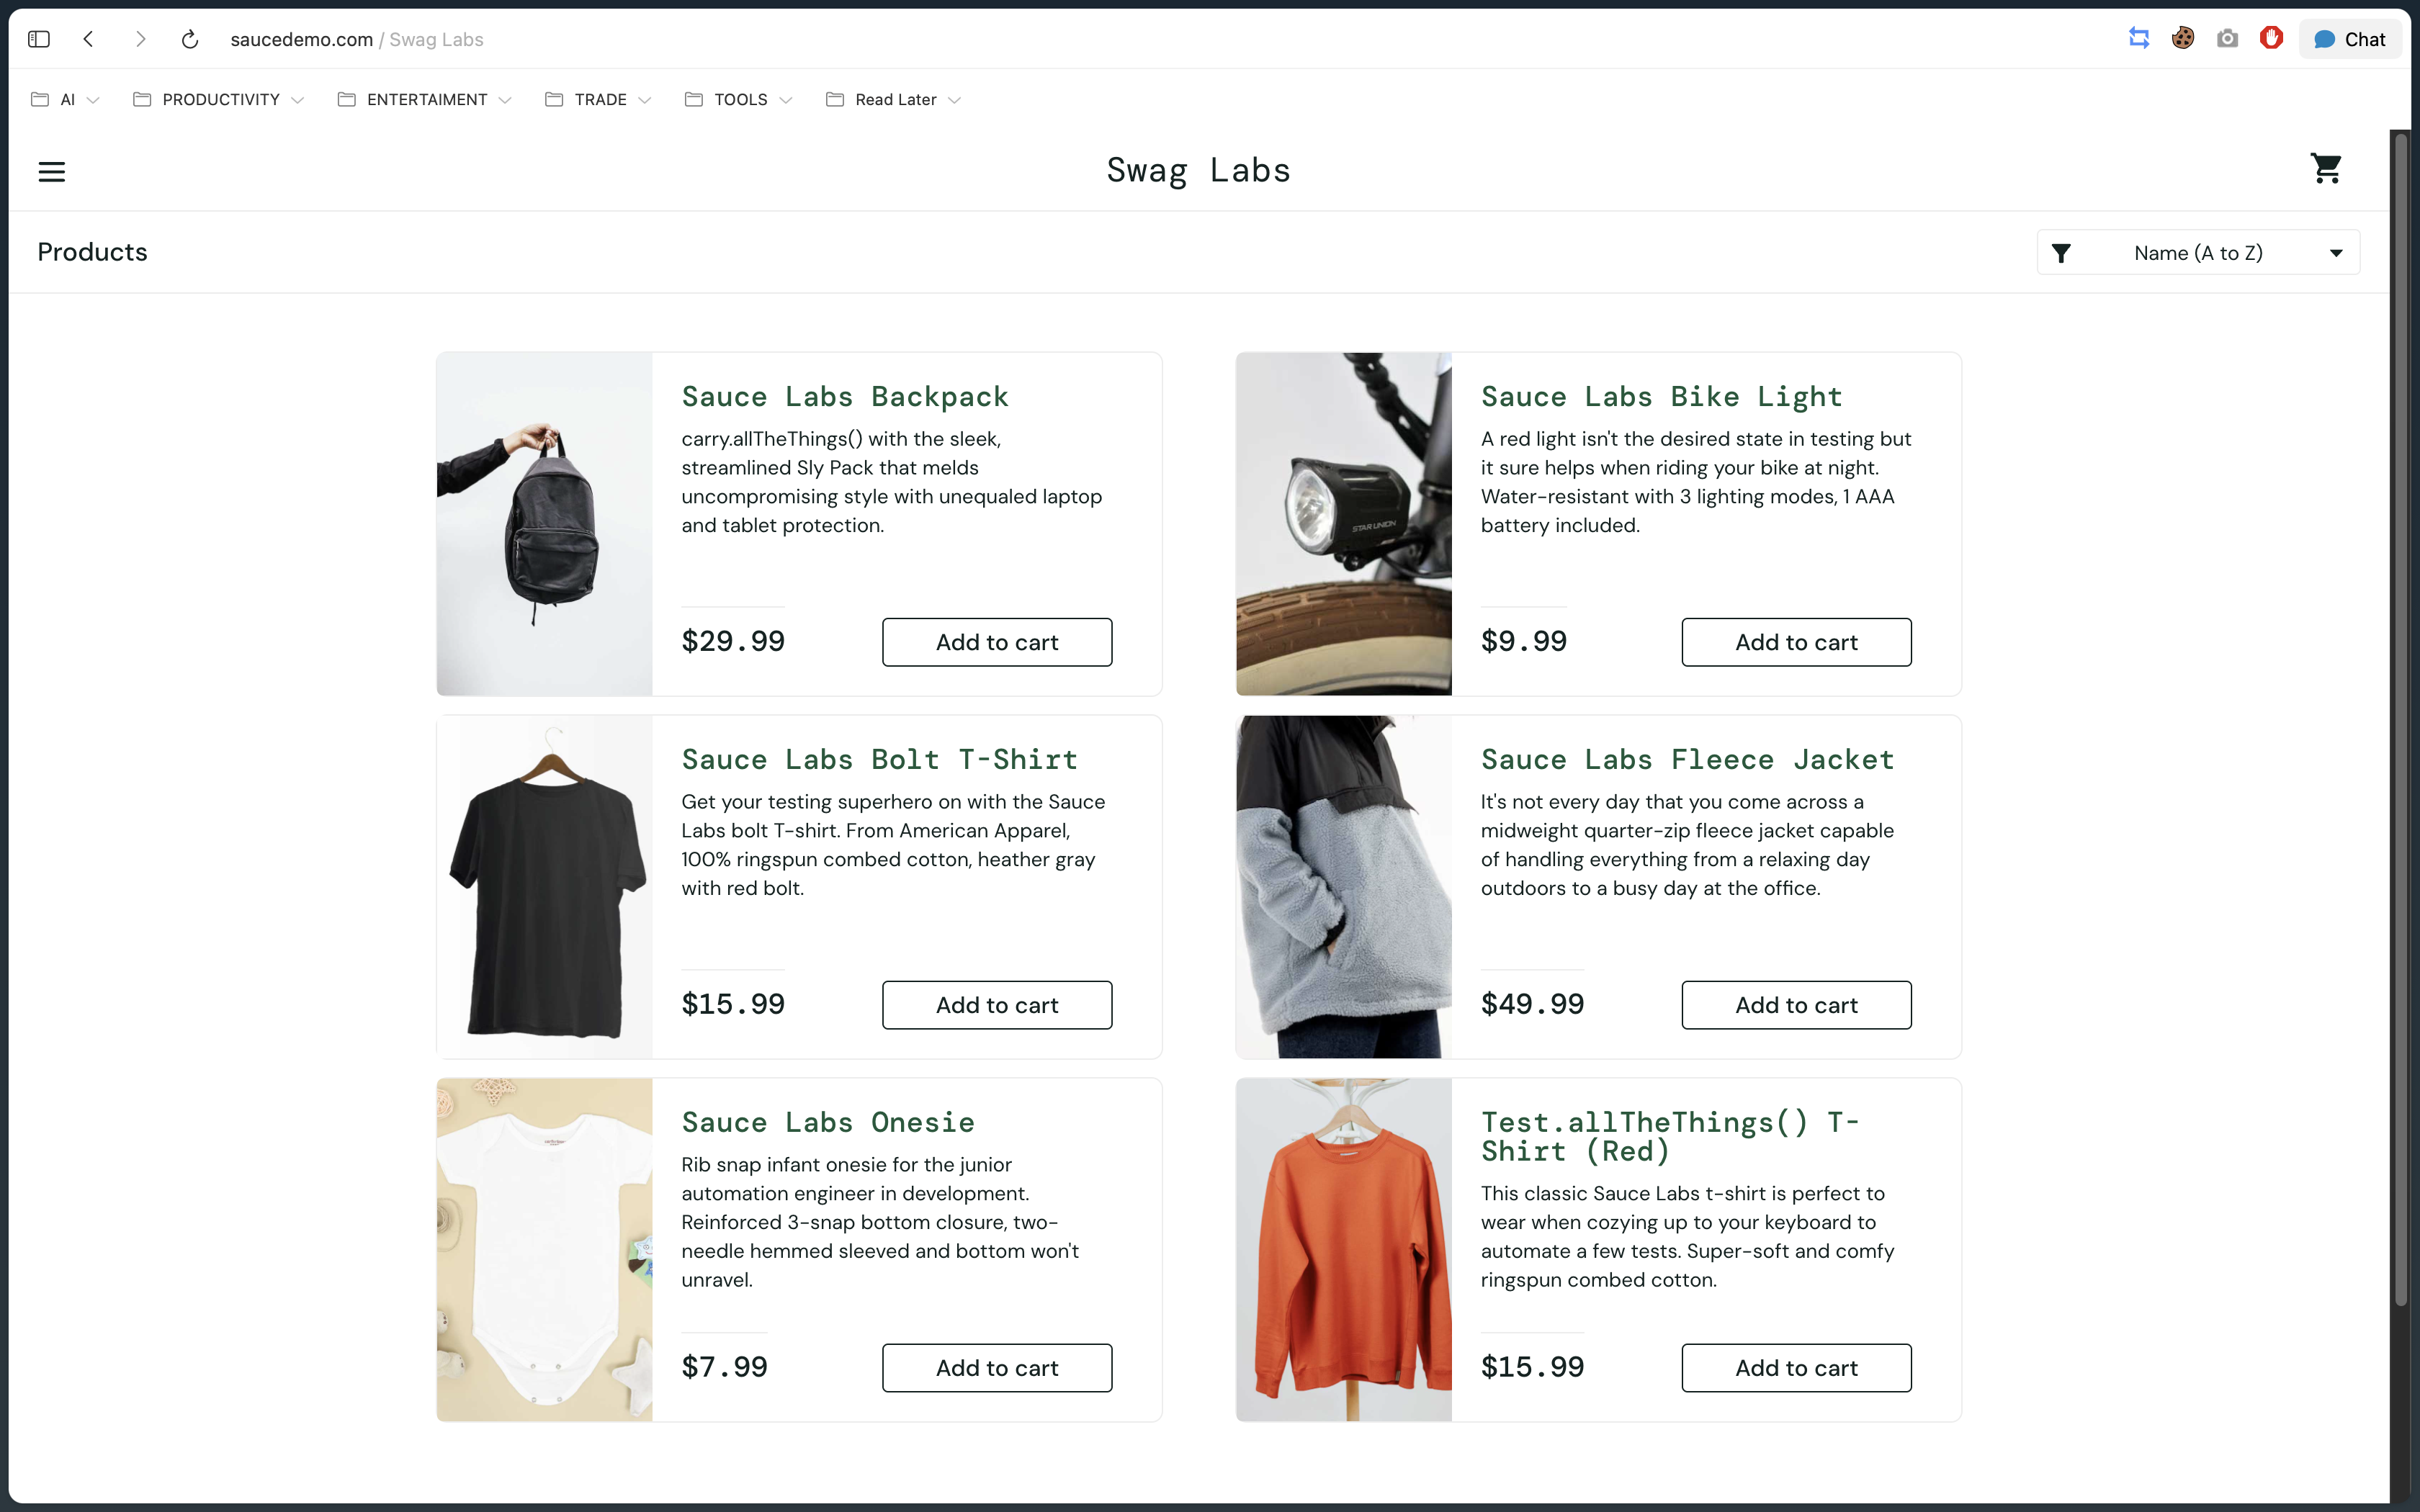
\includegraphics[width=0.9\textwidth]{screenshot step/sauceinventory.png}
    \caption{Hasil Eksekusi Test dengan Implementasi Locators}
\end{figure}

% \chapter{Resources}
% %======================================================================

\section*{Repository}
akses kode lengkap untuk latihan dan tugas praktikum ini dapat ditemukan pada repository GitHub berikut:
\begin{center}
    \href{https://github.com/januarsyah901/PPPL/tree/19b29728e5362f4d3336b97a6b78a093685de30e/Pertemuan%208}{GitHub Repository}
\end{center}

\clearpage

%======================================================================
\chapter{Kesimpulan}
%======================================================================

Berdasarkan praktikum yang telah dilakukan, dapat disimpulkan bahwa penggunaan \textit{kakas bantu} seperti Selenium WebDriver sangat mempermudah pembuatan \textit{automated testing} atau pengujian otomatis antarmuka pada suatu aplikasi secara terstruktur. Pengujian interaksi pada formulir \textit{login} di website \texttt{SauceDemo} dengan mengimplementasikan berbagai \textit{Web Element Locators} (seperti Name, XPath, dan Tag Name) telah berhasil diotomatisasi secara terperinci. 

Selain itu, pendokumentasian skrip pengujian berbasis \textit{Java} serta JUnit telah menunjukkan bagaimana \textit{webdriver} diinstansiasi, dinavigasi mencari \textit{element} dan divalidasi dengan struktur kode secara langsung. Ini sangat menghemat waktu dibandingkan dengan menguji suatu \textit{form login} dan interaksi-interaksi web secara manual berulang-ulang, menstimulasi produktivitas untuk QA (Quality Assurance) serta \textit{Developer} pada tahap-tahap integrasi perangkat lunak nantinya.

% \clearpage
% \addcontentsline{toc}{chapter}{Daftar Pustaka}
% \renewcommand{\bibname}{Daftar Pustaka}

% \begin{thebibliography}{99}
%     \bibitem{mockito} Mockito Project, ``Mockito --- tasty mocking framework for unit tests in Java''. [Online]. Tersedia: \url{https://site.mockito.org/}.
%     \bibitem{junit5} JUnit Team, ``JUnit 5 User Guide''. [Online]. Tersedia: \url{https://junit.org/junit5/docs/current/user-guide/}.
%     \bibitem{fowler-mocks} Martin Fowler, ``Mocks Aren't Stubs'', 2007. [Online]. Tersedia: \url{https://martinfowler.com/articles/mocksArentStubs.html}.
% \end{thebibliography}

\end{document}
